
\documentclass[12pt,a4paper]{article}

\usepackage{rotating}
\usepackage{fancyhdr}
\usepackage{url}
\usepackage{hyperref}
\usepackage{amsmath}
\usepackage{amssymb}
\usepackage{bm}
\usepackage{soul}
\usepackage{graphicx}
\usepackage[cm]{fullpage}
\usepackage{float}
\usepackage{color,soul,xcolor,colortbl}
\usepackage{framed}


%\floatstyle{boxed} 
%\restylefloat{figure}


% \renewcommand{\labelitemi}{$\bullet$}
% \renewcommand{\labelitemi}{$\circ$}
\renewcommand{\labelitemii}{$\circ$}
% \renewcommand{\labelitemii}{$\cdot$}
% \renewcommand{\labelitemiii}{$\diamond$}
% \renewcommand{\labelitemiv}{$\ast$}

\pagestyle{fancy}
\renewcommand{\headrulewidth}{0pt}
\renewcommand{\footrulewidth}{0.3pt}
\fancyhf{}
\lfoot{\footnotesize{Copyright \copyright  \space   \the\year \space The University of Technology Sydney (UTS), Australia.}}
\rfoot{\small{page \thepage}}


\begin{document}


\sethlcolor{yellow}

\pdfpkresolution=2400
\pdfcompresslevel=0
\pdfobjcompresslevel=0
\pdfdecimaldigits=9


\setlength{\parindent}{0pt}
\setlength{\parskip}{2ex}


\begin{titlepage}
\begin{center}


% Title

\vspace*{3cm}

\rule{\linewidth}{0.5mm} \\[0.4cm]
{ \huge \bfseries GMNL2a }\\[0.4cm]
{\large \textsc{GMNL-II with additive approximated afterthought}}

(\textit{a.k.a. OSM -- Offset Scaled Mixed multinomial logit})

{\large \emph{A maximum-likelihood model -- GMNL-II variation on the ``scale vs. preference'' theme.}}
\rule{\linewidth}{0.5mm}
\\[1.1cm]
\large
\textit{Leon(id) Zadorin}
\vspace{3cm}

{\Large \textsc{Centre for the Study of Choice (CenSoC)}}

{\large University of Technology Sydney (UTS), Australia.}


\vfill

\emph{Built from \LaTeX.} \\ 
\InputIfFileExists{git_hash.txt}{\emph{Git-repository contents revision:} \\}{\hl{UNVERSIONED build}}
% {\small \input{git_hash.txt}}

% Bottom of the page
Copyright \copyright  \space   \the\year \space The University of Technology Sydney (UTS), Australia.

\end{center}

\end{titlepage}

\newpage
\tableofcontents
\newpage
\section{Introduction}

At present, this document should invariably be considered a ``work-in-progress'' -- representing a ``thinking out loud'' process where some things could be quite wrong, or they could be correct; the contents could make absolutely no sense or they could lead to a useful model.

Moreover, given that I am not a qualified-scientist -academic -researcher (on subjects such as mathematics, statistics, probability and choice modeling) -- but a software-architect -developer -- any of the content with respect to theoretical propositions and analysis should not be seen a necessarily-endorsed one by (or spoken on behalf of) the university. 

In other words -- ``take it with a grain of salt''.

The document exists for the purposes of transparency and account-keeping so to speak -- it enumerates some of the thoughts and variations on the theme of Generalized Multinomial Logit (GMNL) and, specifically, part thereof: GMNL-II. 

Such variations are conducted in light of attempting to better assimilate any of the numerically-scaled relationships amongst respondents' preferences.

The issues relating to possible misinterpretation of the numerically-scaled relationship for other, non preference-homogeneous, factors are deemed to be outside the scope of this document (and shall, perhaps, be happily addressed later on -- in other ramblings). 

Consequently, as far as this document is concerned -- ``if it looks like a scale then it is a scale'' (i.e. a set of homogeneous preferences).

Moreover, the following choice-characterization of the underlying respondents' data is not aimed at being identified by the Gmnl2a model:
\begin{itemize}
\item ``Distance from zero'' -- the model essentially discards any semantics associated with how close to (or far from) ``zero-line'' the attributes' values happen to be. There is no attempt to identify how confident or unsure respondent preferences happen to be. This, however, may not be so terribly unexpected given that practically any model which deploys random draws (e.g. some form of distribution) will invariably cause movement of the converged-on solution with respect to the aforementioned ``zero-line'' -- based on how much of a numeric ``error'' is caused by the distribution draws. In other words, the ``away from zero'' determination is not only modulated by the error/noise of the unobserved attributes in the utility function, but also by how well the model's noise/random-draws match the underlying dataset -- to such an extent the two aspects may well be ambiguous. This, however, is not seen as the major impediment to identifying heterogeneity of respondents' opinions in the observed dataset (\hl{more on this later}).
\item ``Proportional, inter-attribute relationships'' -- the model does not attempt to preserve/identify the ratio(s) between various attributes. For example, a tuple of attribute values such as \{1, 2\} may easily be transformed into \{0, 1\} thereby causing a different ratio between two attributes. Consequently, those surveys which aim at dealing with such ratios (e.g. willingness to pay) may need to take this point into account. 
\end{itemize}

The Gmnl2a model only concerns itself with a differential relationship between attributes  -- that is to say: ``how much one attribute is more/less important in comparison to another, where importance is essentially a distance between the attributes' beta values''. It is likely that the converged-on values of Gmnl2a model may be normalized/scaled to a given boundary for the purpose of juxtaposition with other models' results -- nevertheless, the notion of differential relationship stands (\hl{more on this later}).

\section{Background}

Given the following characterization of GMNL-II:
{ \Large 
\begin{equation}
U=\sigma(\pmb{\hm{\beta}}+\pmb{\hm{\eta}}) + \varepsilon \label{eq:gmnl_2_1}
\end{equation}
}

where \(\pmb{\hm{\eta}}\) is essentially a \(\pmb{\hm{\sigma}}_{\beta}\), one may see GMNL-II as a rather intuitive mechanism for dealing with numerically-scaled relationship amongst preferences recorded in the underlying dataset (i.e. the semantic preferences of various respondents present in the completed survey's data). Scaled relationship, that is, which was caused by a respondent-specific variation in the amplitude of \(\varepsilon\) -- user's ``sensitivity to the unobserved attributes'' in laymen terms.

The simplification process, when evaluating GMNL-II, may well be extended to a point where one is essentially interested in identifying \textit{only} the \(\hm{\beta}\) and \(\hm{\eta}\). 

The scale distribution (i.e. an outer \(\sigma\) in \autoref{eq:gmnl_2_1}) is, arguably, not so important in it's explicit characterization -- any  account for the actual ``de-scaling'' benefits achieved by GMNL-II could be inferred from a \textit{comparison} of  \(\hm{\eta}\) with that of a traditional mixed logit: \(U=\hm{\beta}+\hm{\eta} + \varepsilon\) where, without the ``scale-absorbing'' \(\sigma\), any of the ``numerically-proportional'' relationships between preferences would be usurped by (or rather attributed to) the \textit{increase across all elements of} \(\hm{\eta}\) as illustrated in \autoref{fig:variances_compared_1} on p.\pageref{fig:variances_compared_1}.


% \begin{sidewaysfigure}
\begin{figure}[H]
\begin{framed}
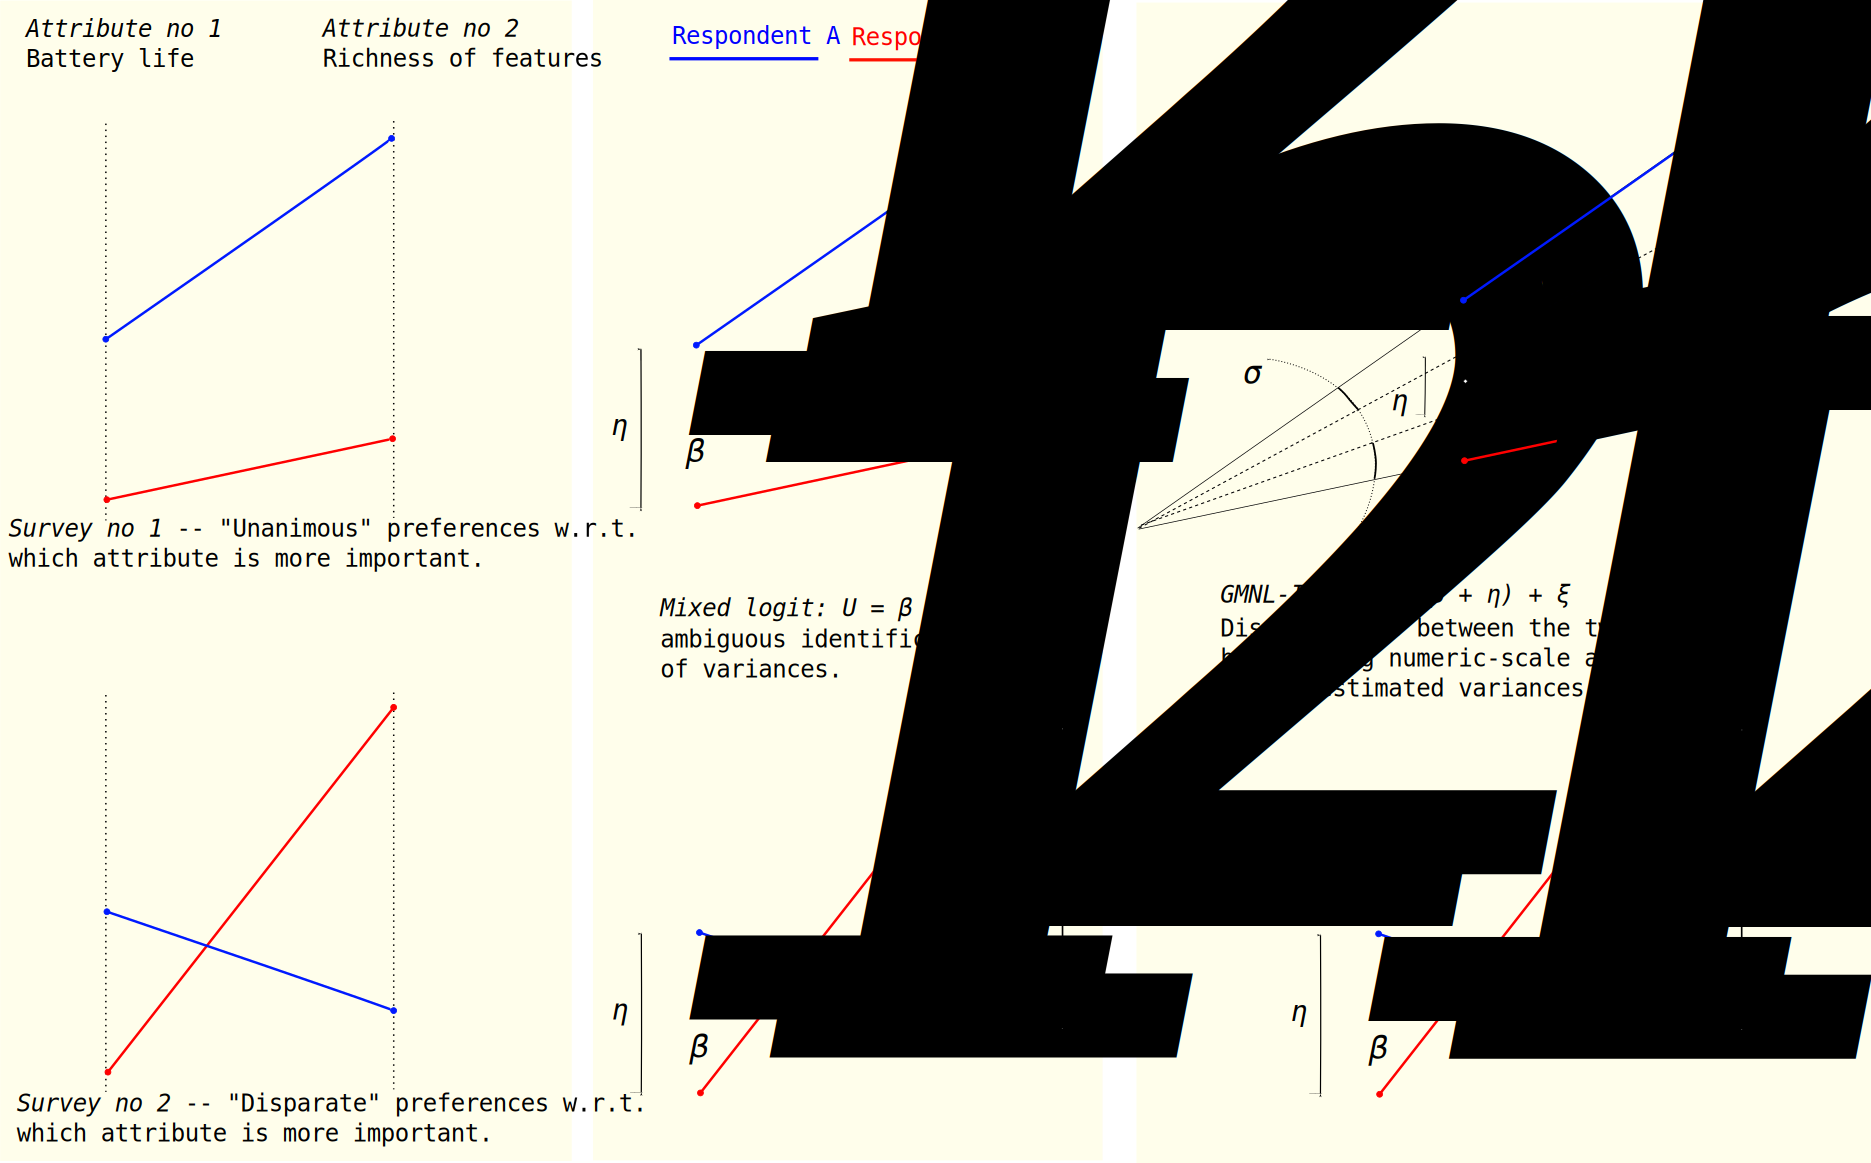
\includegraphics[width=\textwidth, keepaspectratio = true]{pics/intuitive_proposition_1.eps}

Depicts two fictitious surveys for the mobile-phone product where preferences for the battery-life vs the richness-of-features are considered (do presume that each of the respondents has enough observations to have basic logit evaluated individually per respondent).

\caption{Mixed logit vs GMNL-II and relevant (in)ability to separate scale from variance.} 

\label{fig:variances_compared_1}
\end{framed}
\end{figure}
% \end{sidewaysfigure}

In fact, currently-observed empirical results indicate that even in presence of an implicitly ``better fit'' inadvertently introduced by the scaling distribution, the magnitude of heterogeneity in individual attributes  is still retained within \(\pmb{\hm{\eta}}\). \hl{TODO -- more thorough testing}

In other words, even if outer \(\sigma\) is of non-zero value (and at the same time there is no scale relationship among preferences in the underlying dataset), the \(\pmb{\hm{\eta}}\) values \textit{remain} comparatively similar to those from mixed logit analysis, allowing one to leverage such an observation and arrive at a lateral method for scale determination: any underlying presence of homogeneity (i.e. ``true'' scale) is only recognized when all of the \(\pmb{\hm{\eta}}\) values are consistently lower with respect to the \(\pmb{\hm{\eta}}\) values from the corresponding mixed logit analysis. It then becomes, informally speaking, an act of recognizing the explicitly obvious changes in \(\pmb{\hm{\eta}}\)'s elements -- ``the more it looks like a scale, the more likely it is a scale'' type of a generalization.

Conversely, one is, somewhat intuitively, compelled to consider the likelihood of \textit{all of the uncorrelated beta-deviations being \pmb{reduced unanimously and consistentnly}} -- when there is no homogeneous/correlated/synchronized/scale relationship in the underlying respondents preferences -- to be extremely small. \hl{TODO -- more thorough testing, especially w.r.t. identifying cases where there is a priori knowledge of scaled relationships!}

Following the economists' line of reasoning, it is essentially a balance between the importance of the question being answered (i.e. what the survey is for) and the various costs associated with managing the probability of finding a better/more-correct/less-ambiguous answer to the investigated question, especially when such a probability is of a very low value. 

As a minor digression, and possibly an idea for another model, if one is prepared to go further and do attempt to exhaust even the most of the remote possibilities of finding a better, less-ambiguated, solution (i.e. ``just in case it is there'') -- it would behoove one to consider the \textit{SELF-REPLACING} nature of lognormal distribution (\(\ln\mathcal{N}\)) under multiplication. 

In other words, the \(\pmb{\hm{\eta}}\) distribution need not be purely normal (\(\mathcal{N}\)). To begin with, if \(\pmb{\hm{\eta}}\) is simply represented by a \(\ln\mathcal{N}\), then the introduction of an another (outer \(\sigma\)) scaling \(\ln\mathcal{N}\) will not change the nature of a finally-composed distribution: it will remain a lognormal (i.e. \(\ln\mathcal{N}*\ln\mathcal{N}=\ln\mathcal{N}\)).

As a variation to the aforementioned thought, if pure \(\ln\mathcal{N}\) nature of \(\pmb{\hm{\eta}}\) is too awkward/inappropriate then one may specify \(\ln\mathcal{N}*\mathcal{N}\) for \textit{individual} attribute-level distribution draws (i.e. every element of \(\pmb{\hm{\eta}}\) is made up from \(\ln\mathcal{N}*\mathcal{N}\) distribution in both: mixed logit \(U=\hm{\beta}+\hm{\eta} + \varepsilon\) and GMNL-II \(U=\sigma(\hm{\beta}+\hm{\eta}) + \varepsilon\) utility functions). The resulting GMNL-II distribution could then still be reduced as such: \(\ln\mathcal{N}*(\ln\mathcal{N}*\mathcal{N})=\ln\mathcal{N}*\mathcal{N}\)

In other words, a specification is achieved where the scaling distribution can't do anything in terms of ``flexibility-of-fit/distribution-shape'' that the already-existing distributions in \(\pmb{\hm{\eta}}\) could not achieve on their own. The only restriction/decomposition that scaling distribution would impose then would be the ``\textit{synchronous}'' movement of the underlying coefficients. 

The development of such a model, however, is refrained for future musings. This is primarily due to:
\begin{itemize}
\item A relatively low expected lilkelihood of ambiguity (i.e. misinterpretation of a better-fit for the presence of scale) given the requirement for all elements of \(\pmb{\hm{\eta}}\) to be unanimously reduced as per aforementioned explanations. This becomes especially relevant in cases where the survey's attribute levels are further decomposed into attributes in their own right (in terms of the ``vector of observed attributes'' when it comes to their identification in computational models such as mixed logit et. al.) thereby leading to an even greater number of attributes which would be expected to yield a consistent reduction in each of their corresponding variances.
\item At this stage, the main purpose for the Gmnl2a et. al. modeling happens to reside in a role of assistance to the process of identifying various classes/groups of people with homogeneous-to-given-class preferences in a larger dataset. This is generally because any given cumulative/holistic analysis of the whole of the dataset (even with full variance-covariance matrix) is not of much help in determining  homogeneity-of-preference relationships in the face of possibly existing multiple classes/archetypes in the surveyed population. 
\end{itemize}

To bring one's thread-of-thought back to the main context of this rambling, it ought to be mentioned that, naturally, some normalization of the final values is required (due to different ``qualities of fit'' achieved by various models: e.g. mixed logit vs GMNL-II) in order to perform the aforementioned juxtaposition, but more on this later.

Before proceeding any further, it would behoove one to consider how models such as GMNL, mixed logit, et al. actually calculate/determine their parameters during convergence.

The arithmetic of the models appears to be such that it picks only \textit{one} \(\pmb{\hm{\beta}}\) vector as a solution and then, by virtue of some transformation formula, produces a whole \textit{set of transformed beta vectors}. Such a set is then ``tested'' for the likelihood it produces w.r.t. to various respondents' data (i.e. how well all of such transformed beta vectors ``fit'' the data). 

The aforementioned process is usually done many times (each time with a differently picked solution, but with common mechanisms of transformation) and the set yielding the highest likelihood denotes the converged-on parameters for the model. The parameters would include a single vector of betas \(\pmb{\hm{\beta}}\) used to produce the winning set and any other transformation-describing parameters (e.g. scale of the \(\pmb{\hm{\eta}}\) distributions used in the ``transformation'' process).

As an example, consider basic/traditional mixed logit model: \(U=\hm{\beta}+\hm{\eta} + \varepsilon\) (let us suppose that only the uncorrelated \(\mathcal{N}\) distributions for \(\pmb{\hm{\eta}}\) are used in such a model).

The convergence process would essentially start by choosing candidate vectors \(\pmb{\hm{\beta}}\) and \(\pmb{\hm{\eta}}\). Next, for each element of \(\pmb{\hm{\beta}}\), a draw from \(\mathcal{N}\) (with deviation of \(\pmb{\hm{\eta}}\)) will be made and added to the relevant member of \(\pmb{\hm{\beta}}\) resulting in a single instance of the transformed candidate vector. 

In order to generate a whole set of such vectors, the transformation process is repeated many times where candidate vectors do not change (but the values produced by the draws from the distribution obviously vary -- the distribution draws themselves may be done at random or with the help of Halton sequences, etc. but this is largely irrelevant here).

The whole of the resulting set is then tested for the produced likelihood with respect to the underlying survey data.

The key factor in the above descriptions is that only \textit{one} vector of betas (\(\pmb{\hm{\beta}}\)) is picked as the input to the transformation process in order to yield a \textit{set} of transformed betas.

The critical characterization then becomes for the \textit{transformation} process (i.e. a \textit{holistic} mechanism of transformation applied \textit{consistently} to one, single \(\pmb{\hm{\beta}}\)) to produce the best-possible, most-harmonious set of \(\pmb{\hm{\beta}}\)s which would ``fit'' the underlying data (e.g. individual respondents' beta vectors) as much as possible.

Whilst \autoref{fig:variances_compared_1} appears to show no concern for such a requirement for models such as GMNL-II (i.e. its scaling transformation covers all of the underlying preferences reasonably well) the issue becomes more critical if/when \textit{negative} beta values are present in the semantically underlying respondents' preferences as per \autoref{fig:negative_betas_1} p.\pageref{fig:negative_betas_1}. \hl{TODO -- verify that it is indeed infeasible to generate survey datasets where the resulting respondents' betas are all non-negative in the first place...}


\begin{figure}[H]
\begin{framed}
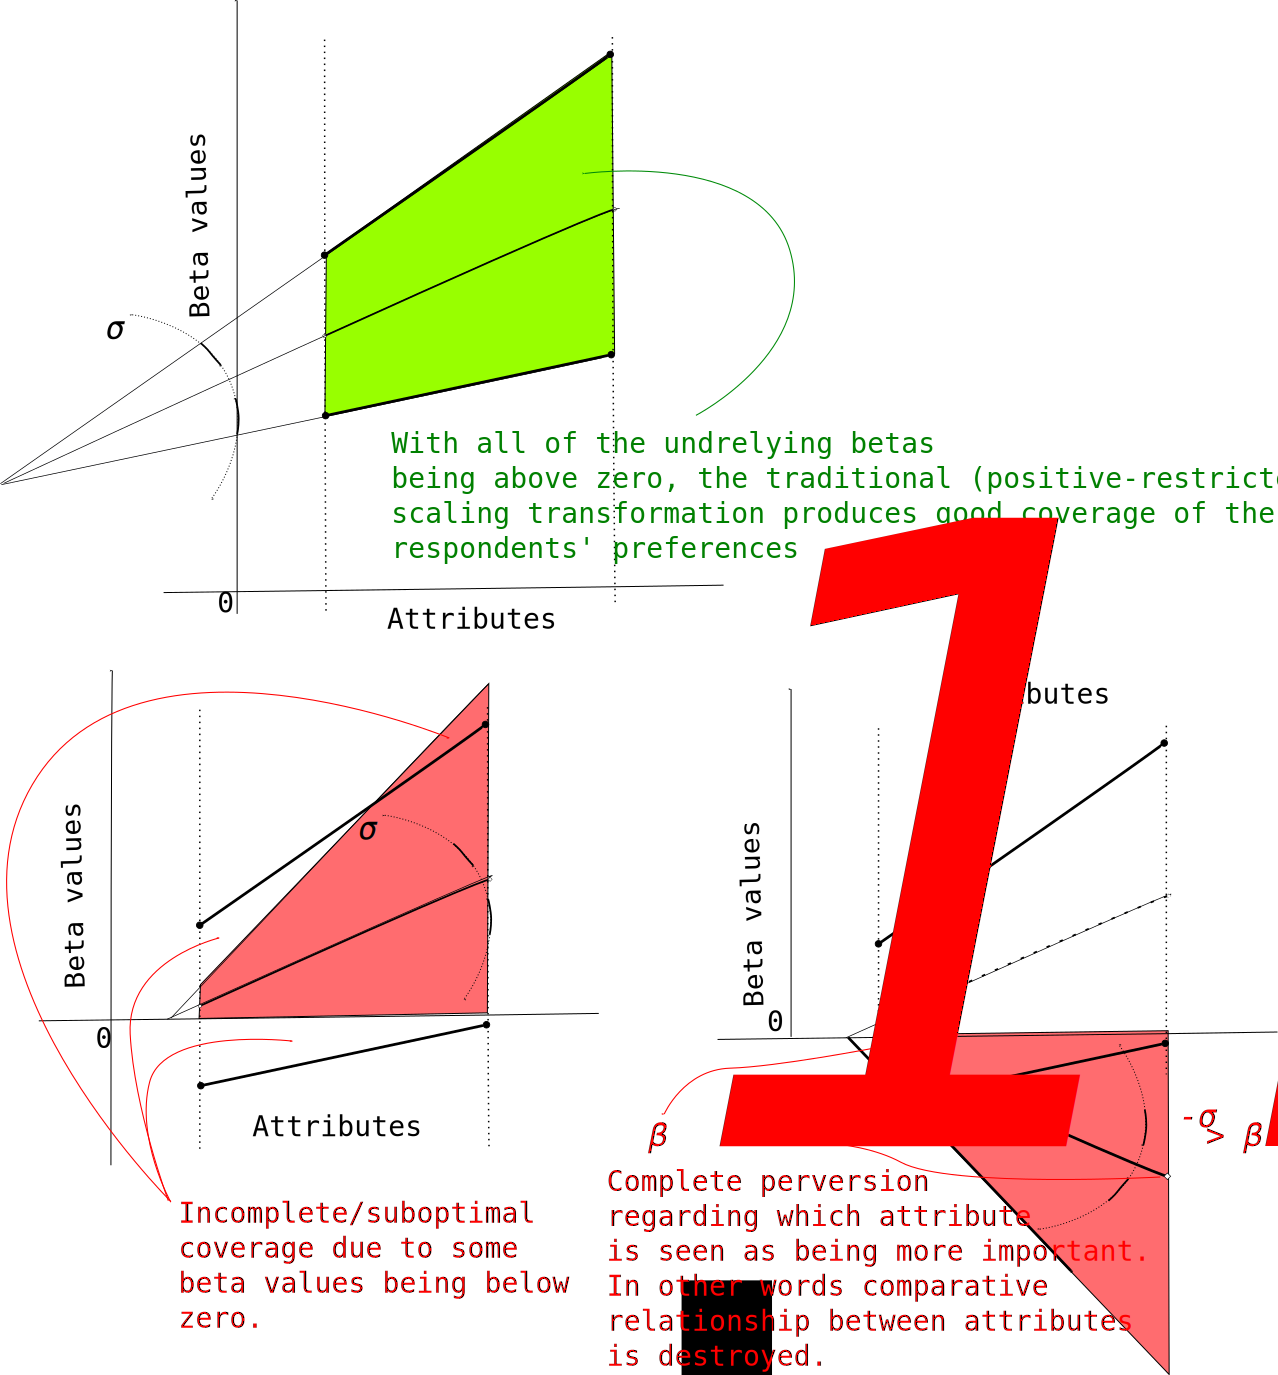
\includegraphics[width=\textwidth, keepaspectratio = true]{pics/negative_betas_1.eps}


\caption{Issues associated with the scaling transformation when some of the underlying betas are negative.} 

\label{fig:negative_betas_1}
\end{framed}
\end{figure}

It might be of interest to momentarily digress and note that mixed logit model is not affected by such a scenario (i.e. it is able to ``fit'' the data equally well irrespective of whether some semantically underlying betas are negative) -- because it's transformation process yields an offsetting/additive process (i.e. distribution draws are \textit{added} to \(\pmb{\hm{\beta}}\)). This points to an auxiliary notion that some transformations are more sensitive to positioning of the underlying betas than others.


\section{GMNL2a}

Given that scaling transformation is at the very center of GMNL-II, one is simply unable to ignore the aforementioned ``negative betas'' difficulties. To such an extent, it is possible to propose a cumulative/holistic offset for the transformational post-processing. 

In other words, the finally-produced set of scale-distributed betas is further transposed up and down before being tested for how well it fits the underlying dataset. 

Figure figure~\ref{fig:gmnl2a_offsetting_1} p.\pageref{fig:gmnl2a_offsetting_1} attempts to illustrate such a visualization.

\begin{figure}[H]
\begin{framed}
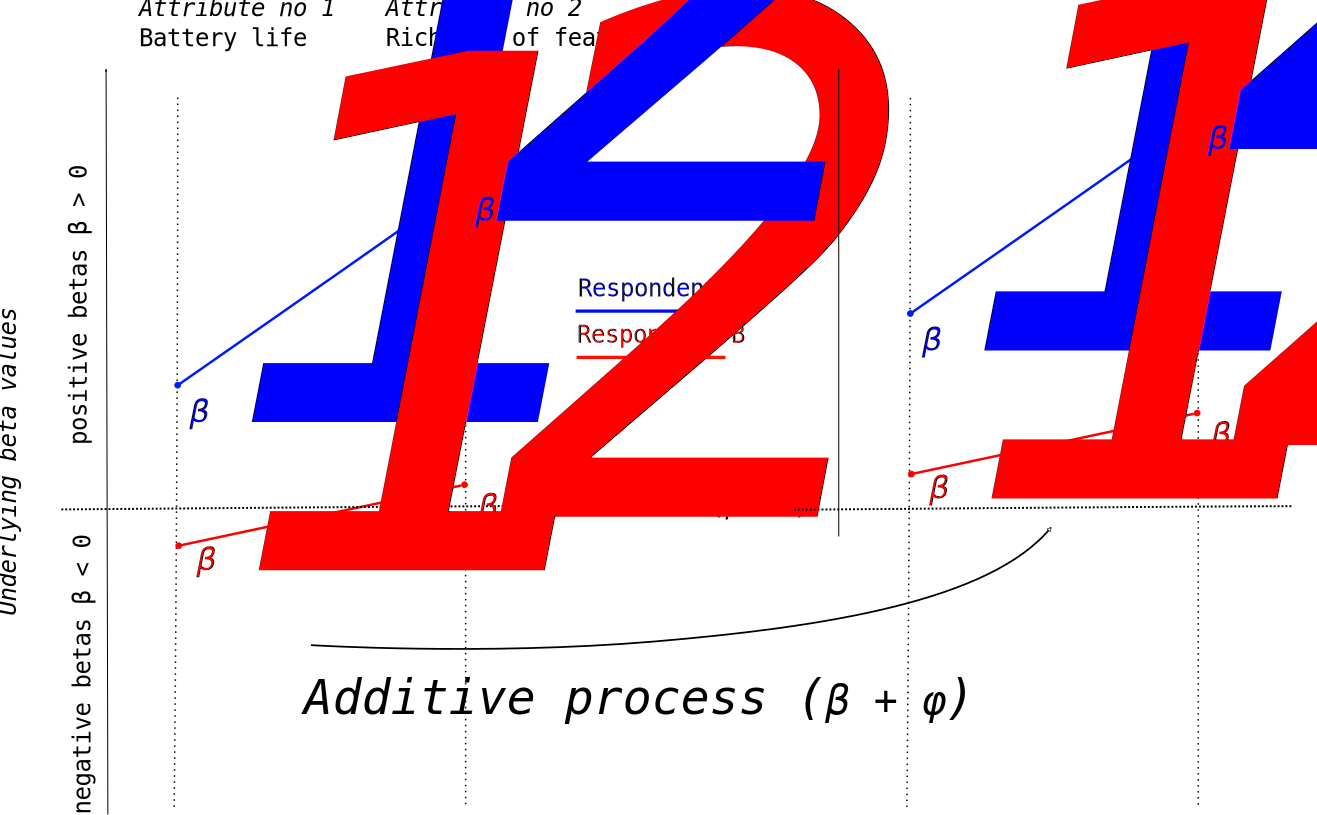
\includegraphics[width=\textwidth, keepaspectratio = true]{pics/gmnl2a_offsetting_1.eps}
\caption{\textit{Additive} post-processing as a part of the transformation process.} 
\label{fig:gmnl2a_offsetting_1}
\end{framed}
\end{figure}

Naturally a more complex localization scenario may be envisaged for the underlying preferences as per \autoref{fig:gmnl2a_offsetting_2}.

\begin{figure}[H]
\begin{framed}
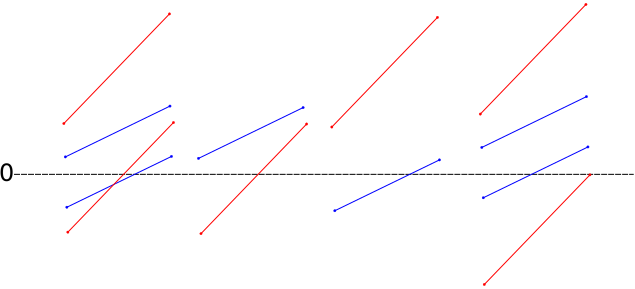
\includegraphics[width=\textwidth, keepaspectratio = true]{pics/gmnl2a_offsetting_2.eps}
\caption{A more complex set of underlying preferences.} 
\label{fig:gmnl2a_offsetting_2}
\end{framed}
\end{figure}

To such an extent the offsetting transformation is currently specified not as a scalar \(\phi\) but rather a distribution \(\Phi\) whose mean, deviation and correlation to the scaling distribution are estimated during a given convergence/terrain-optimization procedure.

The semantic equivalence of the underlying preferences is then seen as a differential relationship between attributes which therefore may undergo holistic scaling transformation without changing their meaning. Likewise, the post-scaling translation of the preferences does not affect their inter-differential relationship.

\subsection{Additive}

The GMNL2a then becomes:
{ \Large 
\begin{equation}
\label{eq:gmnl_2a_1}
U=\Phi + \sigma(\pmb{\hm{\beta}}+\pmb{\hm{\eta}}) + \varepsilon
\end{equation}
}

where the additional scalar \(\phi\) is introduced -- representing an overall additive/subtractive offset for the produced set of transformed betas. 

\subsection{Approximation}

Undoubtedly, however, the offsetting process happens to be an approximation -- the act of moving a whole set of beta vectors up/down in their absolute values is going to compromise any of the existing scale relationships (and possibly introduce some new ones).

For example, given numeric scale between respondents' preferences in the \textit{original} dataset (as illustrated by \autoref{eq:gmnl_2a_2} -- with superscripts denoting respondents and subscripts indicating attributes):

{ \Large 
\begin{equation}
\label{eq:gmnl_2a_2}
\frac{\beta^{^1}_{1}}{\beta^{^2}_{1}}=\frac{\beta^{^1}_{2}}{\beta^{^2}_{2}}
\end{equation}
}

the act of adding just a constant (let alone a whole distribution) to each of the betas may no longer yield the aforementioned (\autoref{eq:gmnl_2a_2}) equivalence as per \autoref{eq:gmnl_2a_3}:

{ \Large 
\begin{equation}
\label{eq:gmnl_2a_3}
\frac{\beta^{^1}_{1} + \bar{\Phi}}{\beta^{^2}_{1} + \bar{\Phi}} \neq \frac{\beta^{^1}_{2} + \bar{\Phi}}{\beta^{^2}_{2} + \bar{\Phi}}
\end{equation}
}

Such a compromise, however, is not expected to be of significant detriment in a multitude of practically-feasibly scenarios.

\subsection{Afterthought}

With respect to the GMNL model, and it's underlying theoretical foundations, \(\Phi\) is really an afterthought -- in that it does not feature explicitly at the theoretical level, but rather at the stage of numeric ``fitting'' considerations/challenges when converging on the aggregated set of multiple respondents' preferences.

\subsection{Post-convergence normalization}

After convergence is completed there is a need to counter any of the offsets/``distortions'' produced by the aforementioned modulation, or indeed to simply manage a different ``quality of fit'' as compared to other models whose absolute/raw solutions may be higher/lower with respect to a zero-line orientation (i.e. certainty/uncertainty indicator, which in our case is discarded anyways). 

Generally speaking, the following process is applied in order to produce parameters (\(\pmb{\hm{\beta}}\) and \(\pmb{\hm{\eta}}\)) to be of comparable values when compared to other, similar to GMNL2a, models (e.g. GMNL-I, GMNL-II, mixed logit and so on):

\begin{itemize}

\item \(\sigma\) and \(\Phi\) are discarded (as per the aforementioned GMNL-II simplification notion)

\item the resulting \( \pmb{\hm{\beta}} \) and \( \pmb{\hm{\eta}} \) are normalized -- each element of the aforementioned vector is scaled by a constant. The constant value is determined in such a way that the normalization process makes the absolute difference between the largest and lowest element of \( \pmb{\hm{\beta}} \) equal to \(1\). 

\item at this stage \( \pmb{\hm{\eta}} \) are considered to be normalized, whilst \( \pmb{\hm{\beta}} \) elements are shifted so as to reside between \(0\) and \(1\).

\end{itemize}

Such a normalization process is envisaged to be applied to other, comparable, models (e.g. \( \pmb{\hm{\beta}} \) and \( \pmb{\hm{\eta}} \) in mixed logit). This allows for cross-model comparison with respect to obtained attribute-preferences within a group of respondents and their respective heterogeneity of the opinion (i.e. variances).

For example, given the following ``raw'' estimated parameters:

\begin{itemize}
\item \(\pmb{\hm{\beta}} = \{2, 1, 3, 5\}\)
\item \(\pmb{\hm{\eta}} = \{0.5, 3, 2, 0.1\}\)
\end{itemize}

the ``massaged'' output would be generated in the following manner:

\begin{itemize}
\item Obtain normalization constant \(1 / (5 - 1) =\frac{1}{4}\)
\item Scale both the \( \pmb{\hm{\beta}} \) and \( \pmb{\hm{\eta}} \) by \(\frac{1}{4}\)
\item \(\pmb{\hm{\beta}} = \{0.5, 0.25, 0.75, 1.25\}\)
\item \(\pmb{\hm{\eta}} = \{0.125, 0.75, 0.5, 0.025\}\)
\item then further offset to reside between zero and one \(\pmb{\hm{\beta}} = \{0.5 - 0.25, 0.25 - 0.25, 0.75 - 0.25, 1.25 - 0.25\} = \{0.25, 0, 0.5, 1\}\)
\end{itemize}

In a similar fashion, if a different model (e.g. mixed logit) had converged on the same dataset with the following ``raw'' parameters:

\begin{itemize}
\item \(\pmb{\hm{\beta}} = \{-1.5, -3, 0, 3\}\)
\item \(\pmb{\hm{\eta}} = \{1, 6, 4, 0.2\}\)
\end{itemize}

Then it's normalization process would yield:
\begin{itemize}
\item Obtain normalization constant from betas \(1 / (3 - -3) = \frac{1}{6}\)
\item Scale both the \( \pmb{\hm{\beta}} \) and \( \pmb{\hm{\eta}} \) by \(\frac{1}{4.5}\)
\item \(\pmb{\hm{\beta}} = \{-0.25, -0.5, 0, 0.5\}\)
\item \(\pmb{\hm{\eta}} = \{0.167, 1, 0.67, 0.033\}\)
\item then further offset to reside between zero and one \(\pmb{\hm{\beta}} = \{-0.25 + 0.5, -0.5 + 0.5, 0 + 0.5, 0.5 + 0.5\} = \{0.25, 0, 0.5, 1\}\)
\end{itemize}

Finally two models would be juxtaposed with respect to their parameters (e.g. \(\pmb{\hm{\eta}}\) values) as per \autoref{fig:normalized_values_comparison_1}. 


\begin{figure}[H]
\begin{framed}
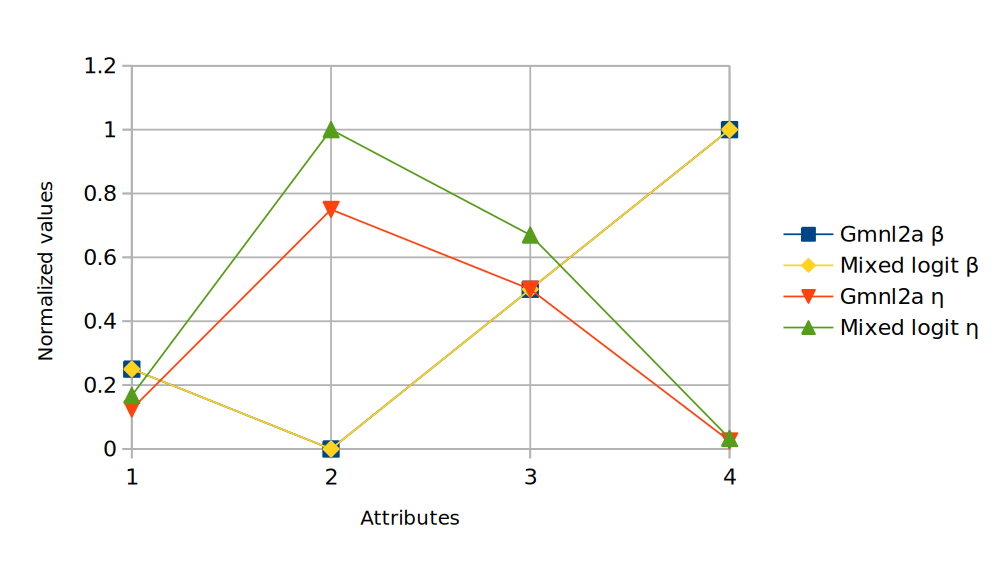
\includegraphics[width=\textwidth, keepaspectratio = true]{pics/normalized_values_comparison_1.eps}
\caption{Juxtaposed models.} 
\label{fig:normalized_values_comparison_1}
\end{framed}
\end{figure}


Naturally, the aforementioned example is rather contrived, but the thesis of the intent for the post-normalization process remains. In essence, the ``zero to one'' normalization of \( \pmb{\hm{\beta}} \) values is arbitrary (e.g. corresponding \( \pmb{\hm{\eta}} \) values may well end up being outside such a range), and a different scalar value may be chosen -- for as long as such remains consistent with respect to all of the compared models and is applied to all of the  \( \pmb{\hm{\beta}} \) and \( \pmb{\hm{\eta}} \) elements.

\end{document}
